\begin{figure}[ht]
\begin{center}
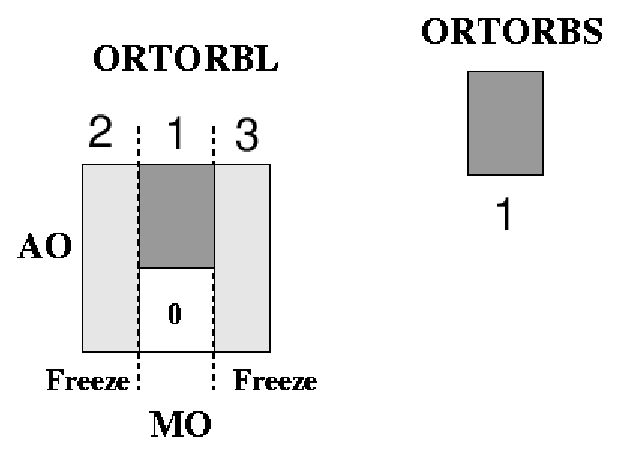
\includegraphics[width=7cm,keepaspectratio]{02_localization/images/matrix-2.eps}
\caption{\footnotesize A visual representation of the hierarchical
orthonormalization performed on the orbitals. The non-frozen orbitals
(marked with ``1'' in figure) are orthonormalized among themselves.
Then, frozen core orbitals (marked with ``2'' in figure) are orthonormalized
among themselves and against the non-frozen ones. Finally, the frozen
virtual orbitals (marked with ``3'') are orthonormalized against ``1'' and ``2''.
}
\label{fig:matrix-2}
\end{center}
\end{figure}

